

\chapter{Hybrid Encryption}
	
\begin{itemize}
	\item Public Key Encryption is expensive
	\item 2-3 orders of magnitude slower than private key encryption
	\item AES Encryption rate: $\sim 700MB/s$ per core
	\item RSA Encryption rate: $\sim 1.5MB/s$ per core
	\item How can we efficiently encrypt large amounts of data?\\
	$\Rightarrow$ Combine public and private key encryption to get the best of both!
	\item Idea: For every encryption, generate a fresh $K$ key for a private key encryption scheme
	\item Use $K$ to encrypt the payload message
	\item Encrypt $K$ using a public key encryption scheme
\end{itemize}
\begin{center}
	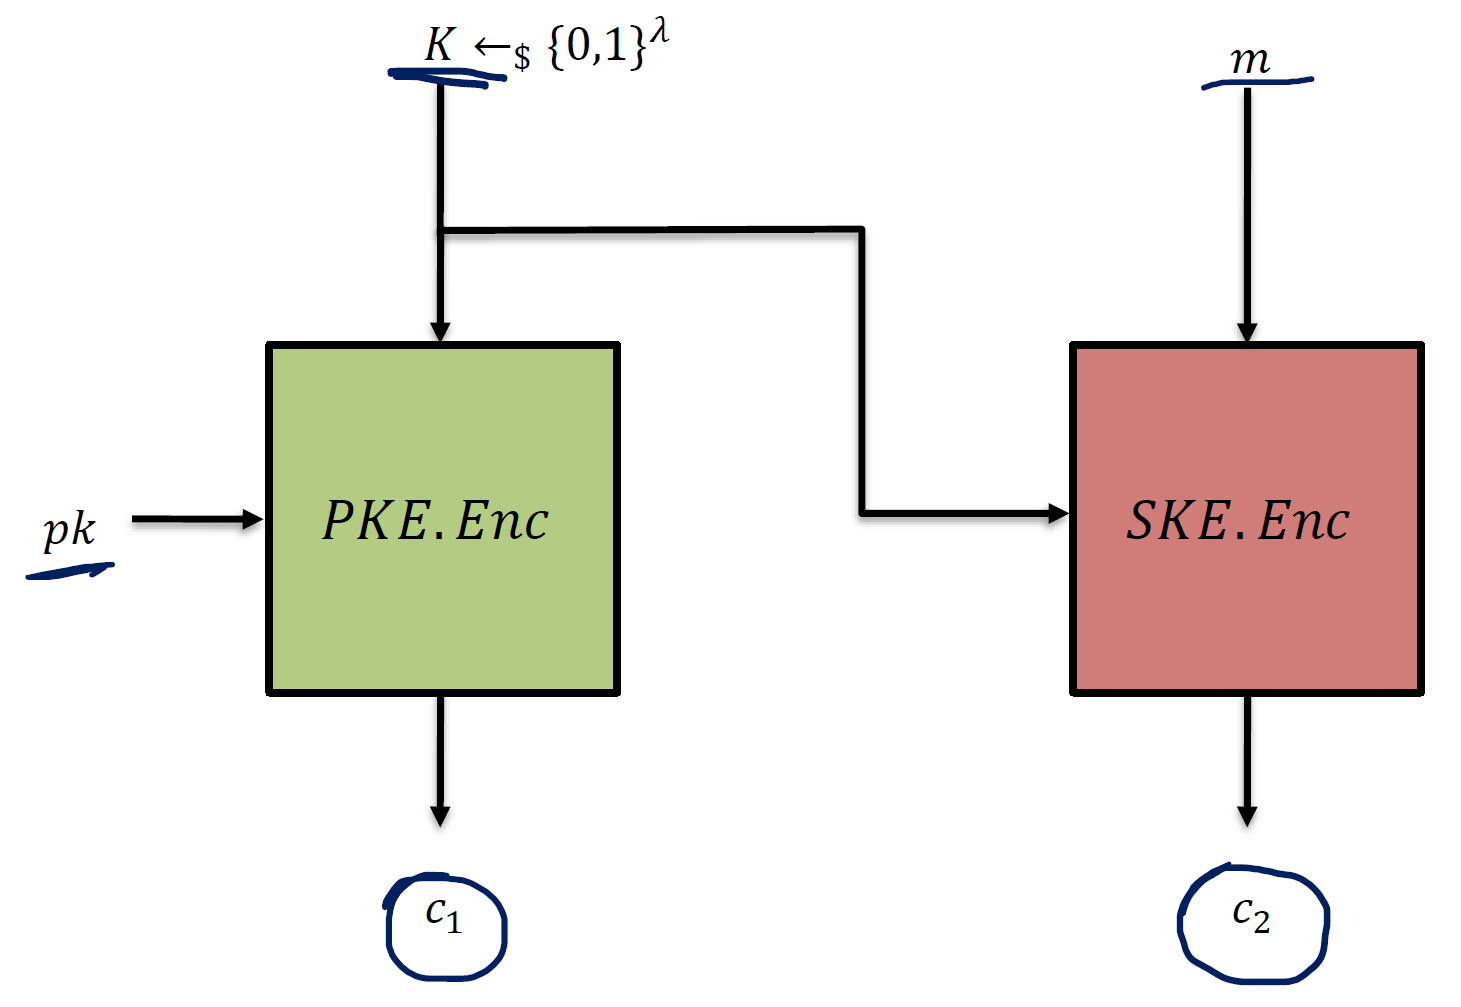
\includegraphics[width=120mm]{Graphics/Hybrid Encryption/he1.png}
\end{center}

\section{Advantages of Hybrid Encryption}
	\begin{itemize}
		\item Key $K$ is short, e.g. 256 bits
		\item Thus expensive public key operation only performed once for a very short message
		\item The bulk of work is performed by the \textit{fast} private key encryption scheme
		\item Also minimizes the size of the ciphertext for large messages $\rightarrow$ saves bandwidth
		\item For private key encryption $|c_2| \approx |m|$
		\item Thus $\frac{|c|}{|m|} \approx \frac{|c_1|+|m|}{|m|} = \frac{|c_1|}{|m|} + 1 \approx 1$
	\end{itemize}
	\begin{center}
		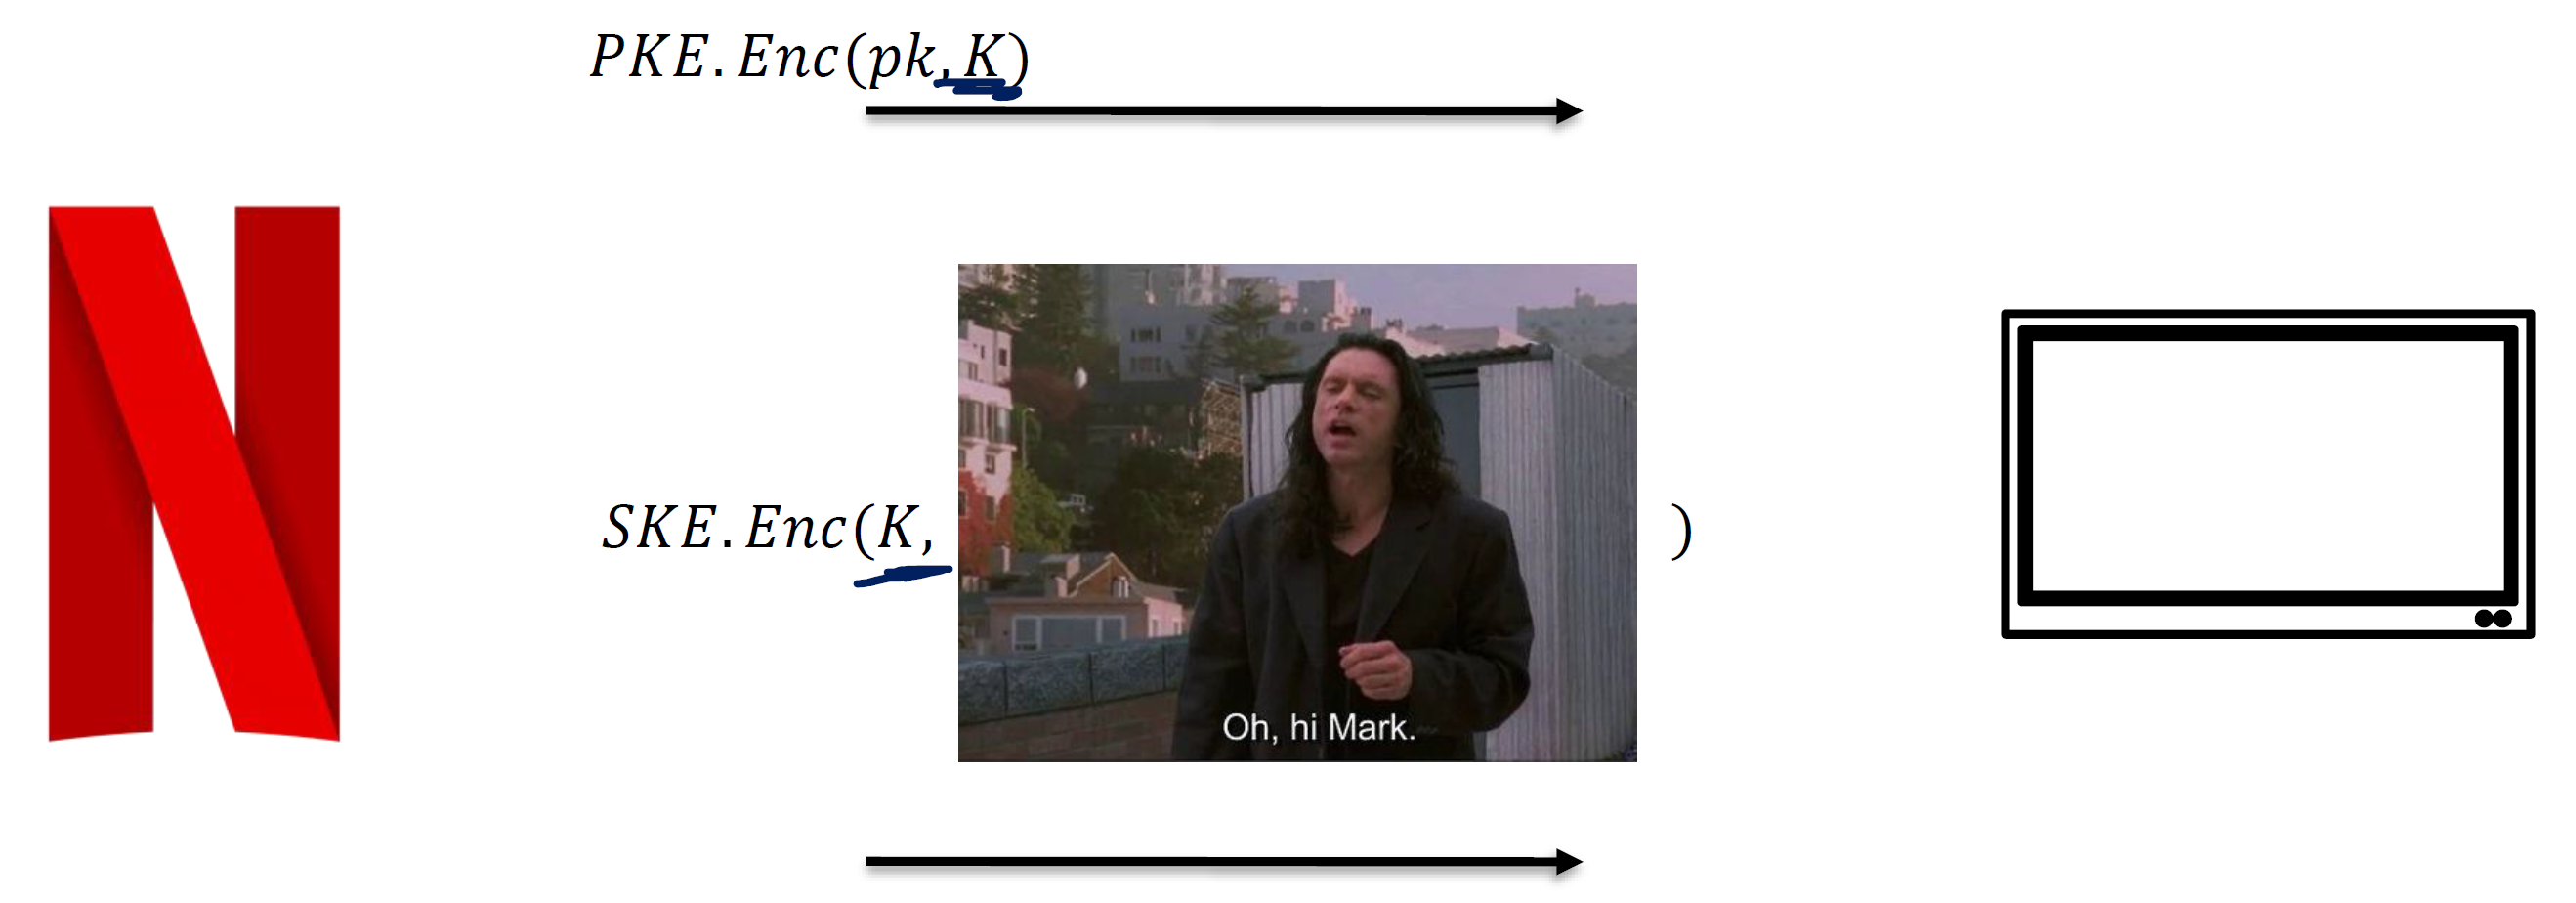
\includegraphics[width=120mm]{Graphics/Hybrid Encryption/he2.png}
	\end{center}

\section{Key Encapsulation}
	\begin{itemize}
		\item Using public key encryption this way, the ciphertext $c_1$ merely \textit{encapsulates} a randomly chosen key $K$
		\item Key Encapsulation Mechanism (KEM):\\
		Replace (public key) encryption algorithm by an algorithm which generates a key $K$ together with a ciphertext $c$ which encapsulates $K$
		\item This allows for small (e.g. factor $\sim 2$) size and efficiency improvement, as ciphertext doesn’t need to encode arbitrary user-chosen messages
	\end{itemize}
	\begin{center}
		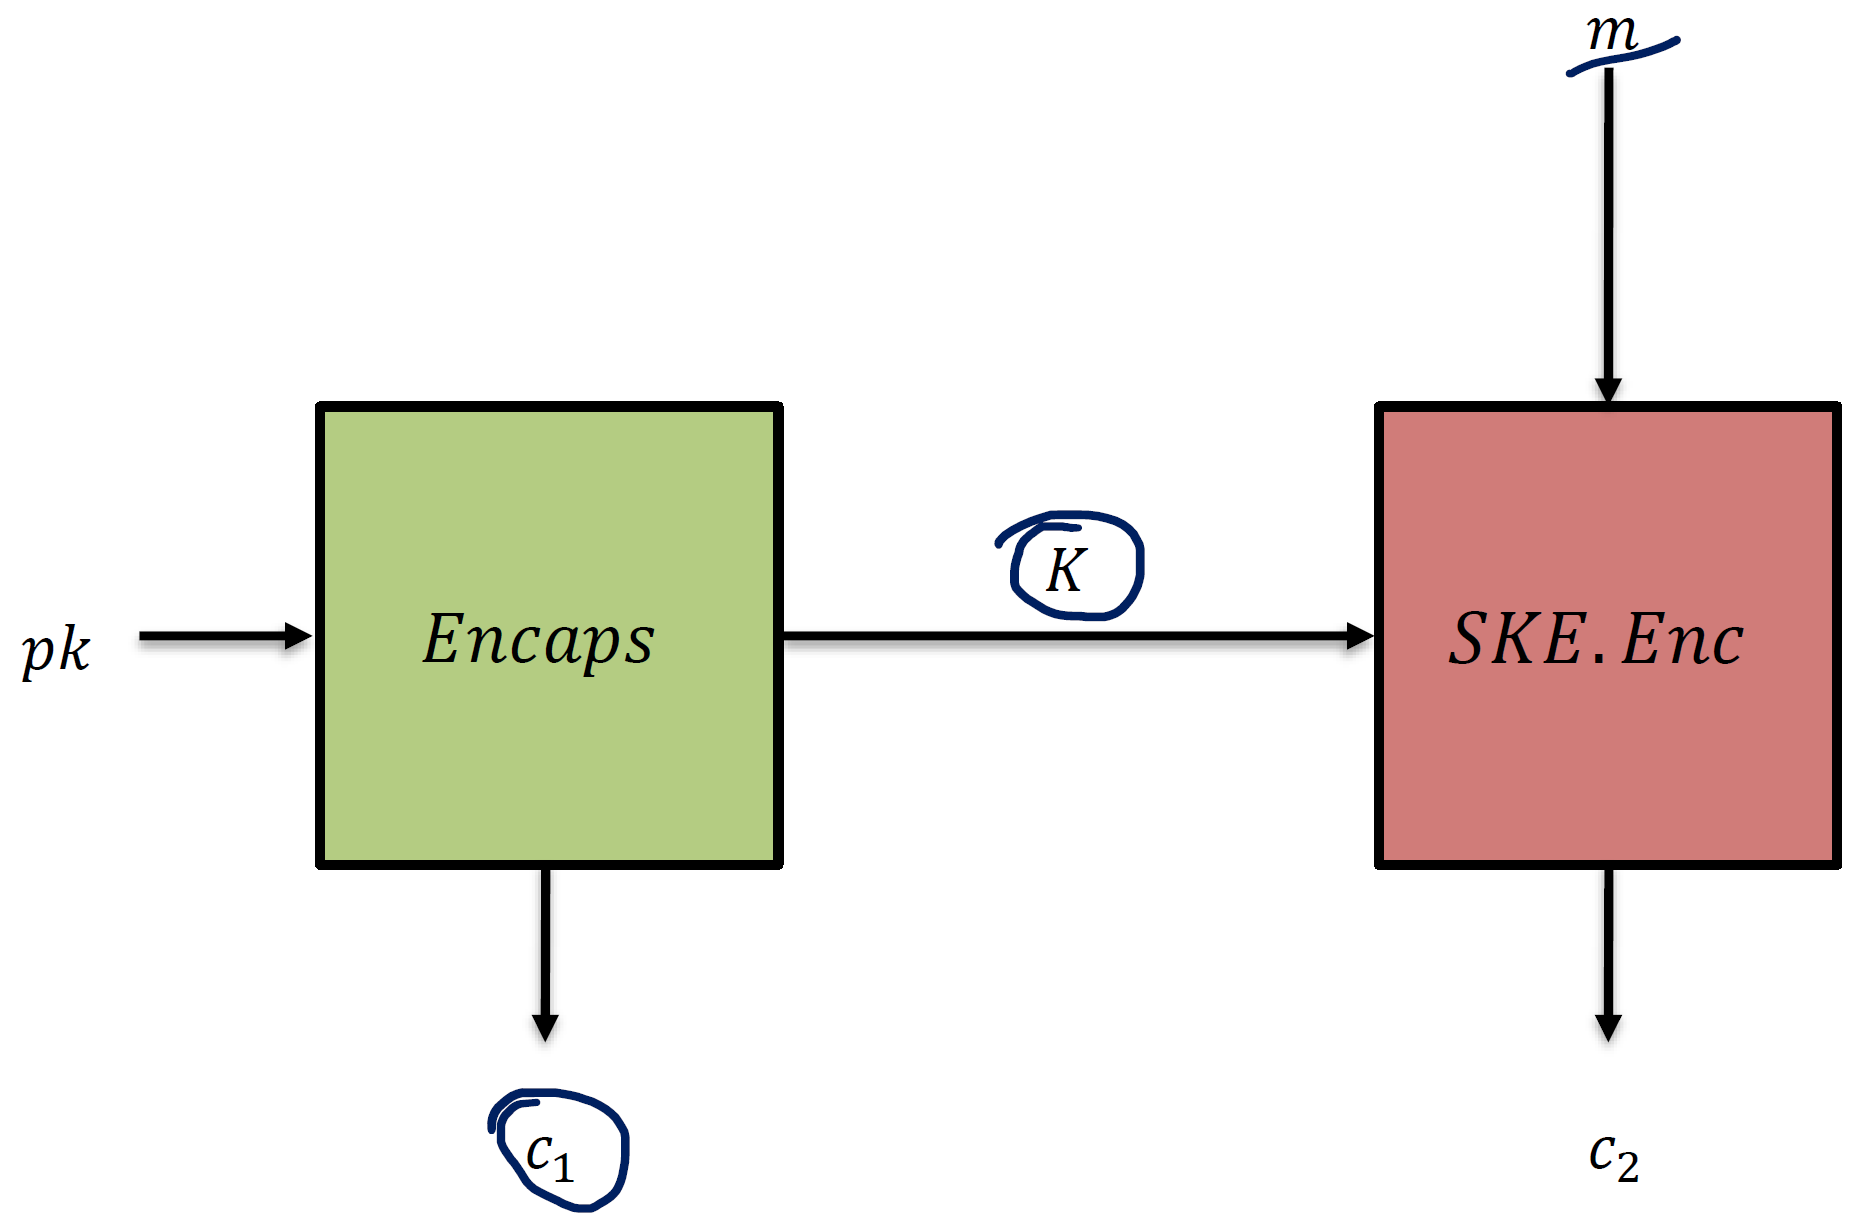
\includegraphics[width=120mm]{Graphics/Hybrid Encryption/he3.png}
	\end{center}

\section{Key Encapsulation Mechanisms}
	\textbf{Syntax:} A key encapsulation mechanism (KEM) consists of three PPT algorithms: $(KeyGen,Encaps,Decaps)$
	\begin{itemize}
		\item $KeyGen(1^{\lambda})$: A randomized algorithm which takes as input the security parameter $1^{\lambda}$ (encoded in unary) 
		and outputs a pair of \textbf{public} and \textbf{secret} keys $(pk,sk)$
		\item $Encaps(pk)$: A randomized algorithm which takes a public key $pk$ and outputs a ciphertext $c$ and a key $K$
		\item $Decaps(sk,c)$: A deterministic algorithm which takes as a secret key $sk$ and a ciphertext $c$ as input and outputs a key $K$
	\end{itemize}
	\textbf{Correctness:} It holds for all $\lambda \in \mathbb{N}$ that $Pr[Dec(sk,c)=K]=1$, where $(pk,sk) \leftarrow KeyGen(1^{\lambda})$ and $(c,K) \leftarrow Encaps(pk)$

\section{CPA Security for KEMs}
	\begin{definition}
		A KEM $(KeyGen,Encaps,Decaps)$ is $IND-CPA$\textbf{-secure}, if it holds for \textbf{every PPT-adversary} $\mathcal{A}$ 
		there exists a negligible function $v$ s.t. for all $\lambda \in \mathbb{N}$
		$$Pr[IND-CPA_{\mathcal{A}}(\lambda)=1] < \frac{1}{2} + v(\lambda)$$
	\end{definition}
	\begin{center}
		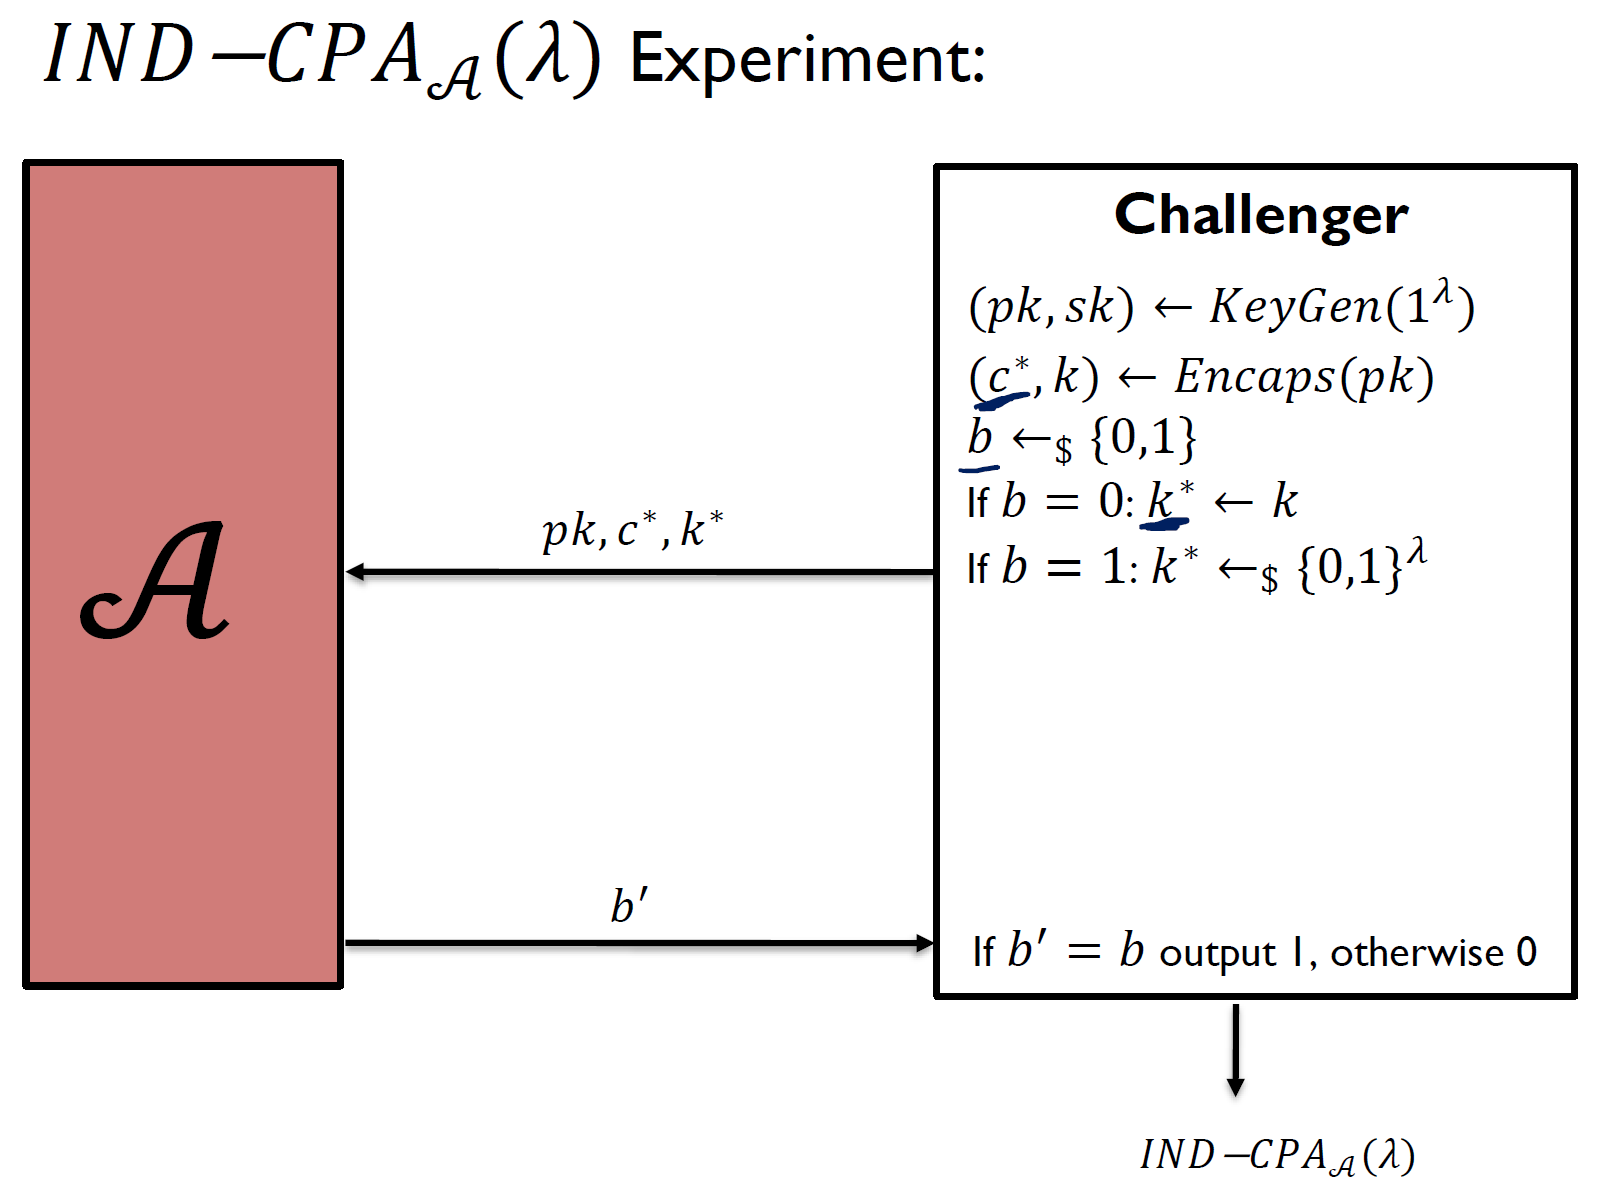
\includegraphics[width=120mm]{Graphics/Hybrid Encryption/he4.png}
	\end{center}

\section{Examples of KEMs}
	\begin{itemize}
		\item Trivial KEM: Use PKE to encrypt key $K$
		\begin{itemize}
			\item $Encaps(pk)$: Choose $K \leftarrow_{\$} \{0,1\}^{\lambda}$, compute $c \leftarrow Enc(pk,K)$ and output $(c,K)$
			\item $Decaps(sk,c)$: Compute and output $K \leftarrow Dec(sk,c)$
		\end{itemize}
		\item Every 2-message key exchange protocol immediately yields a KEM
		\item Example: Diffie-Hellman KEM
		\begin{itemize}
			\item $KeyGen(1^{\lambda})$: Choose $x \leftarrow_{\$} \mathbb{Z}_p$, compute $h \leftarrow g^x$, outout $pk \leftarrow (g,h)$ and $sk \leftarrow x$
			\item $Encaps(pk)$: Choose $y \leftarrow_{\$} \mathbb{Z}_p$, compute and outout $c \leftarrow g^y$ and $K \leftarrow h^y$
			\item $Decaps(sk,c)$: Compute and output $K \leftarrow c^x$
		\end{itemize}
		\item Ciphertext is only one group element (ElGamal: 2 group elements)
		\item IND-CPA security follows immediately from eavesdropping security of Diffie-Hellman key exchange (the two experiments are identical)
	\end{itemize}

\section{Public Key Encryption from KEM + Private Key Encryption}
	\begin{itemize}
		\item We will now show that the above construction actually yields an IND-CPA secure encryption scheme
		\item Let $(KeyGen,Encaps,Decaps)$ be a KEM and $(Enc,Dec)$ be a private key encryption scheme (with uniformly random keys).
		The public key encryption scheme $(KeyGen',Enc',Dec')$ is given as follows
		\begin{itemize}
			\item $KeyGen'(1^{\lambda})$: Compute and output $(pk,sk) \leftarrow KeyGen(1^{\lambda})$
			\item $Enc(pk,m)$: Compute $(C_1,K) \leftarrow Encaps(pk)$, $c_2 \leftarrow Enc(K,m)$ and output $c \leftarrow (c_1,c_2)$
			\item $Dec(sk,c=(c_1,c_2))$: Compute $K \leftarrow Decaps(sk,c_1)$, compute and output $m \leftarrow Dec(K,c_2)$
		\end{itemize}
	\end{itemize}

\section{$IND-CPA$ Security}
    \begin{theorem}\label{thm8.3}
        \item Assume that $(KeyGen,Encaps,Decaps)$ is an $IND-CPA$ secure $KEM$
        \item Assume further that $(Enc,Dec)$ is an $IND$ secure provate key encryption scheme
        \item Then $(KeyGen',Enc',Dec')$ is an $IND-CPA$ secure public key encryption scheme
    \end{theorem}
    \begin{proof}
        Assume $\mathcal{A}$ is a PPT adversary with non-negligible advantage $\epsilon$ against the $IND-CPA$ security of $(KeyGen',Enc',Dec')$.\\\\
        \textbf{\underline{Goal:}} Show that this implies that either $(KeyGen,Encaps,Decaps)$ is not $IND-CPA$ secure, or $(Enc,Dec)$ not $IND$-secure.
        $IND-CPA$ Experiment for $(KeyGen',Enc',Dec')$
    	\begin{center}
    		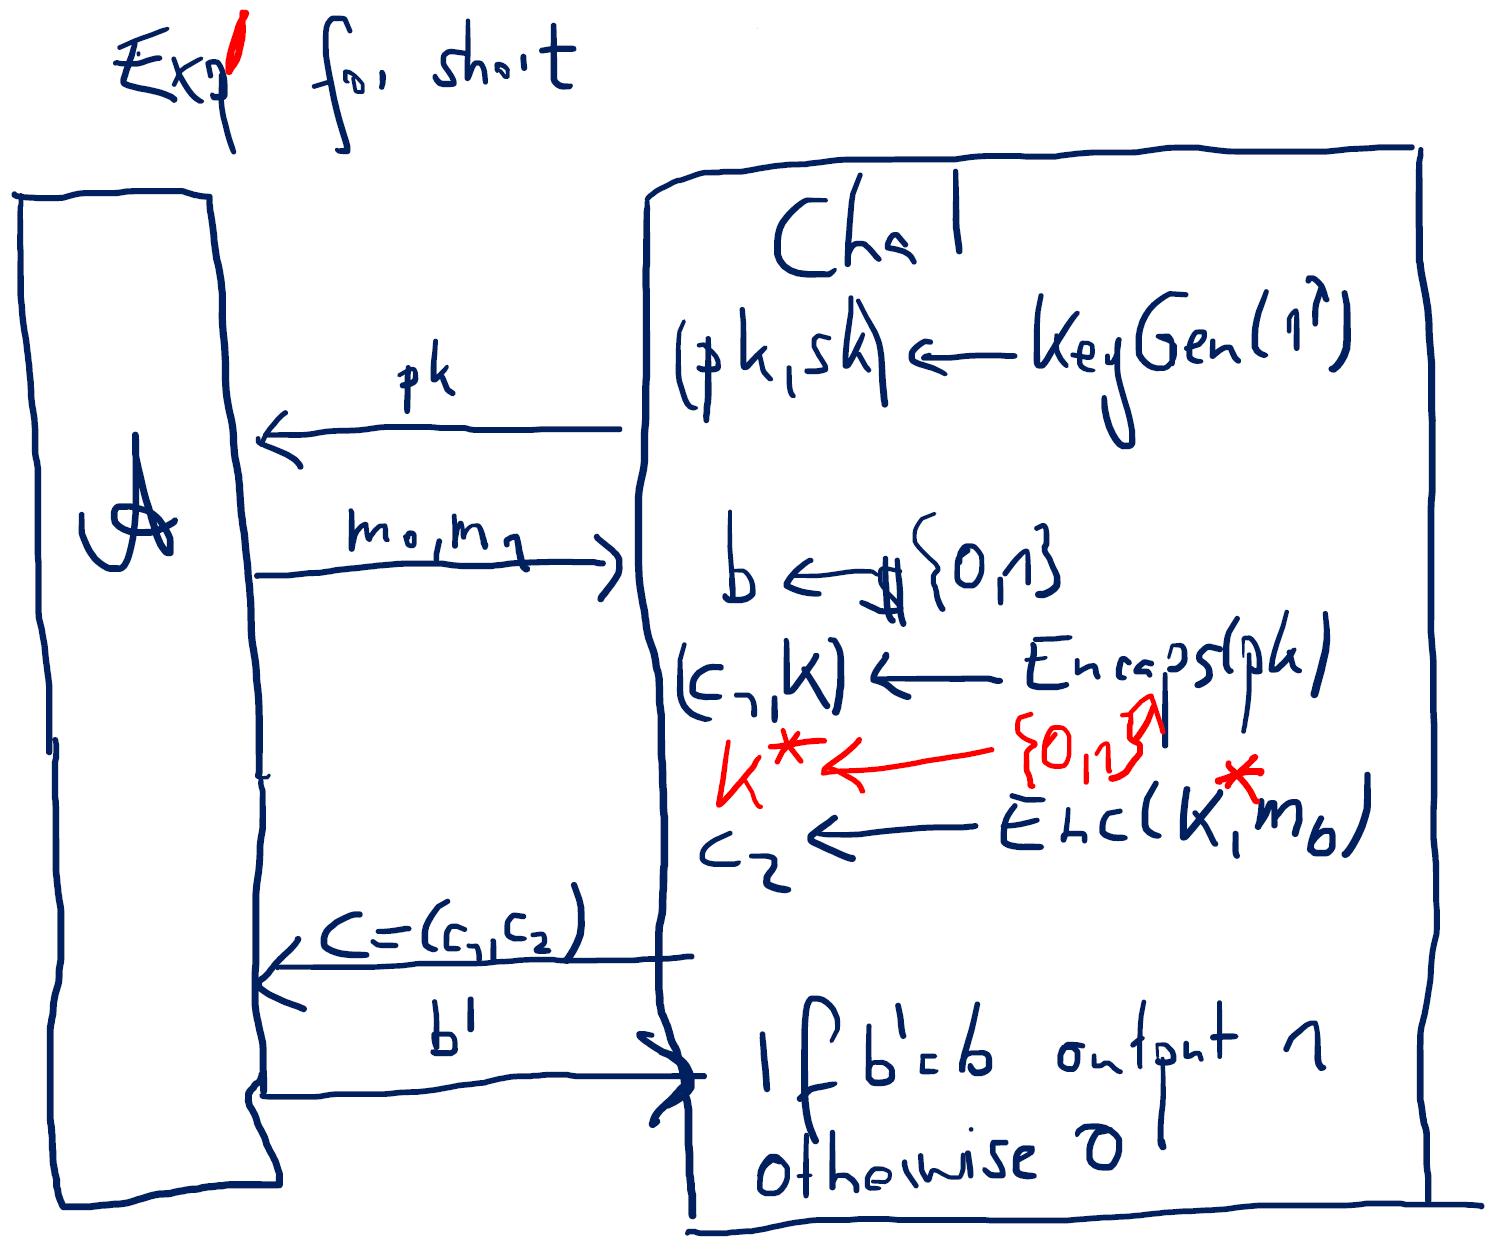
\includegraphics[width=160mm]{Graphics/Hybrid Encryption/he5.png}
    	\end{center}
    	\textbf{\underline{Claim:}}
    	    $$|Pr[Exp'=1]-Pr[Exp=1]| < negl.$$
    	Proof of Claim:\\
    	Assume towards contradiction that
    	$$|Pr[Exp'=1]-Pr[Exp=1]| > \epsilon'$$
    	for a non-negligible $\epsilon'$\\
    	We will construct a PPT adversary $\mathcal{A}'$ with advantage $\epsilon'$ against $IND-CPA$ security of $KEM$
    	\begin{center}
    		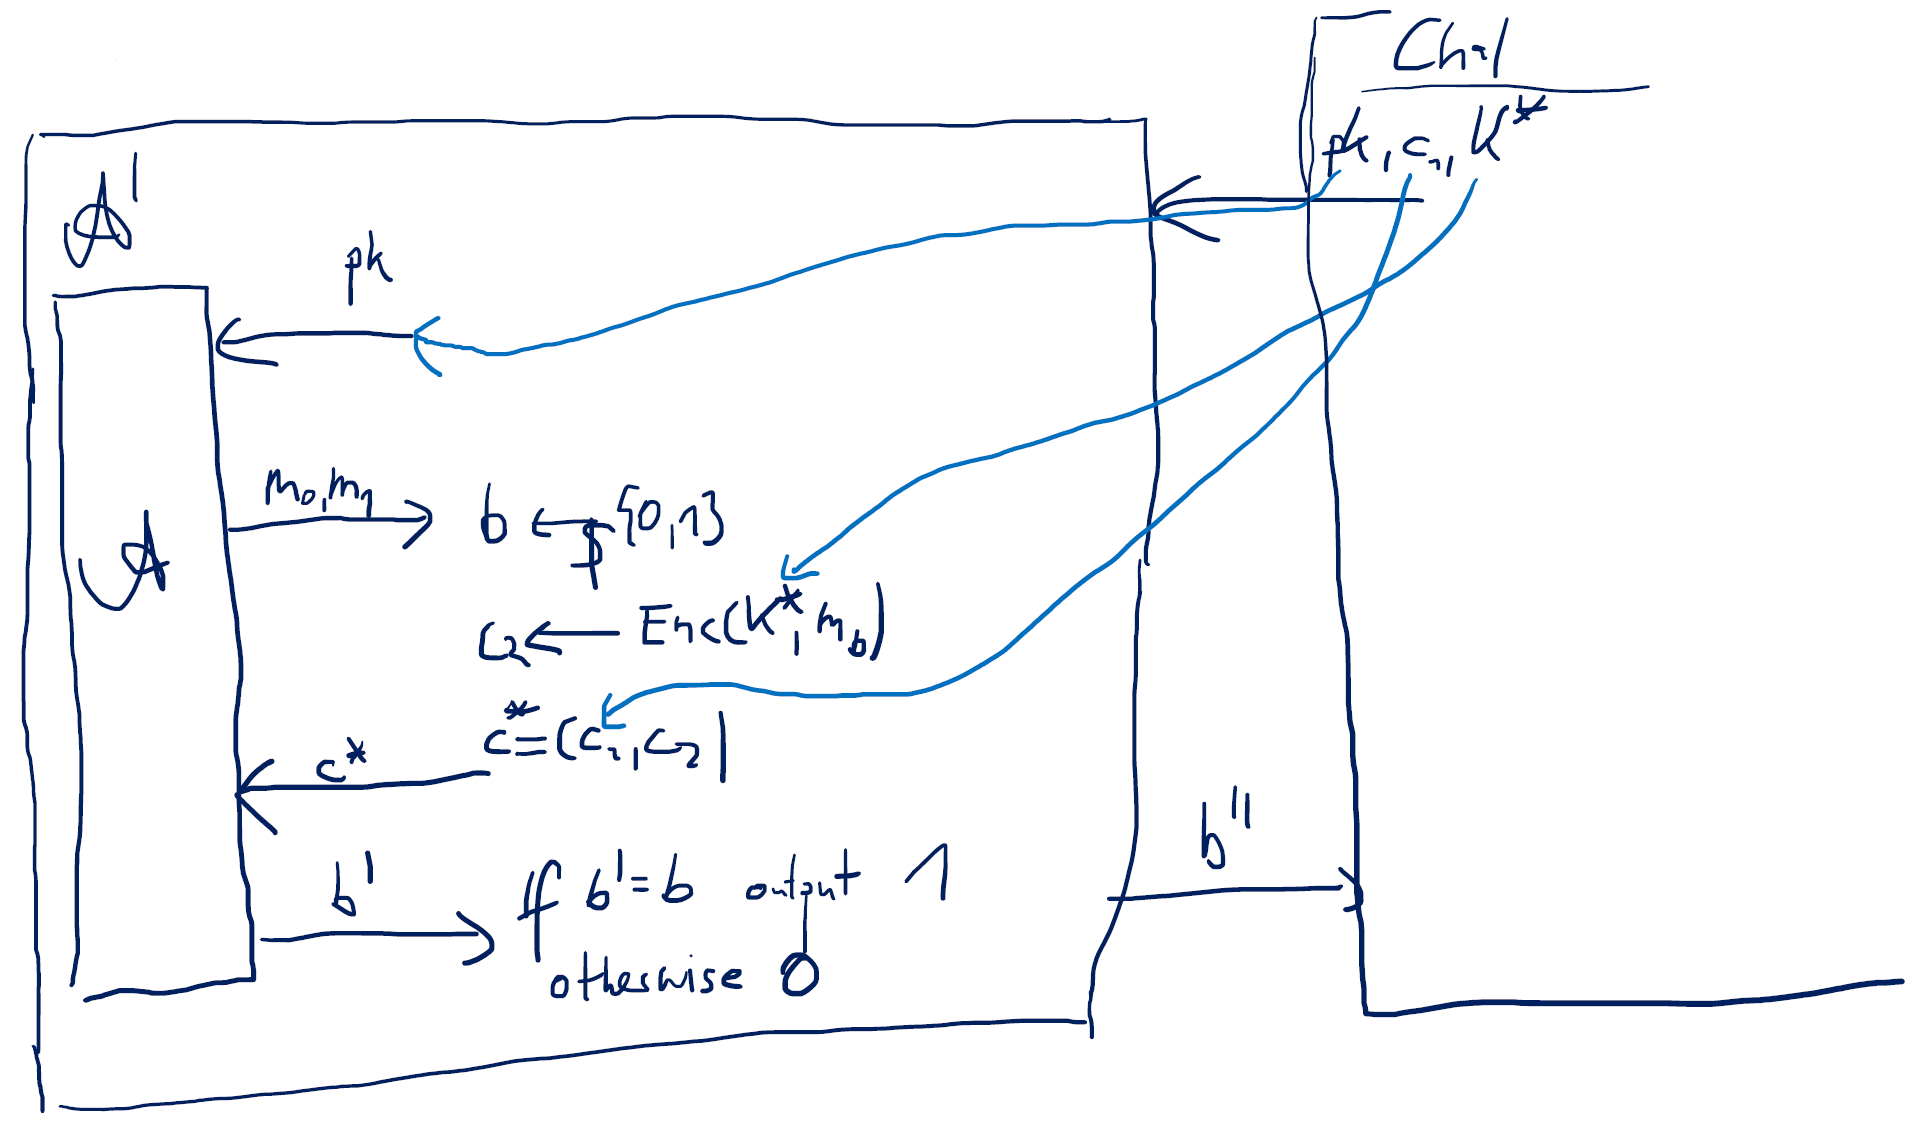
\includegraphics[width=160mm]{Graphics/Hybrid Encryption/he6.png}
    	\end{center}
    	Let $b^*$ be the challenge-bit of $\mathcal{A}'$ challenger.\\\\
    	\textbf{\underline{Case 1:}} $b^* = 0$\\
    	In this case input $(pk,c_1,k^*)$ of $\mathcal{A}'$ was computed by $(c_1,k^*) \leftarrow Encaps(pk)$\\
    	$\Rightarrow$ $\mathcal{A}'$ faithfully simulates $Exp$ from the view of $\mathcal{A}$\\
    	$\Rightarrow$ $Pr[IND-CPA_{\mathcal{A}}(\lambda)=1 \mid b^*=0] = Pr[Exp=0]$\\\\
    	\textbf{\underline{Case 1:}} $b^* = 1$\\
    	In this case $(pk,c_1,k^*)$ is computed by $(c,k) \leftarrow Encaps(pk)$ and $k^* \leftarrow \{0,1\}^{\lambda}$\\
    	$\Rightarrow$ In this case $\mathcal{A}'$ faithfully simulates $Exp'$ from the view of $\mathcal{A}$\\
    	$\Rightarrow$ $Pr[IND-CPA_{\mathcal{A}'}(\lambda)=1 | b^*=1] = Pr[Exp'=1]$
    	\begin{align*}
    	    Pr[IND-CPA_{\mathcal{A}'}(\lambda)=1] &= \frac{1}{2} \cdot \underbrace{Pr[IND-CPA_{\mathcal{A}'}(\lambda) \mid b^*=0]}_{=Pr[Exp=0]=1-Pr[Exp=1]} 
    	                                           + \frac{1}{2} \cdot \underbrace{Pr[IND-CPA_{\mathcal{A}'}(\lambda) \mid b^*=1]}_{=Pr[Exp'=1]}\\
    	                                          &= \frac{1}{2} + \frac{1}{2} \cdot \underbrace{|Pr[Exp'=1]-Pr[Exp=1]|}_{\geq \epsilon'} \geq \frac{1}{2} + \frac{\epsilon'}{2}
    	\end{align*}
    	contradicts $IND-CPA$ security of $KEM$
    	Consequently: 
    	    $$Pr[Exp'=1] \geq \underbrace{\frac{1}{2} + \epsilon - negl.}_{\epsilon''}$$
    	We will now show that this implies a PPT adversary $\mathcal{A}''$ with adversary $\epsilon''$ against $IND$-security of $(Enc,Dec)$.
    	\begin{center}
    		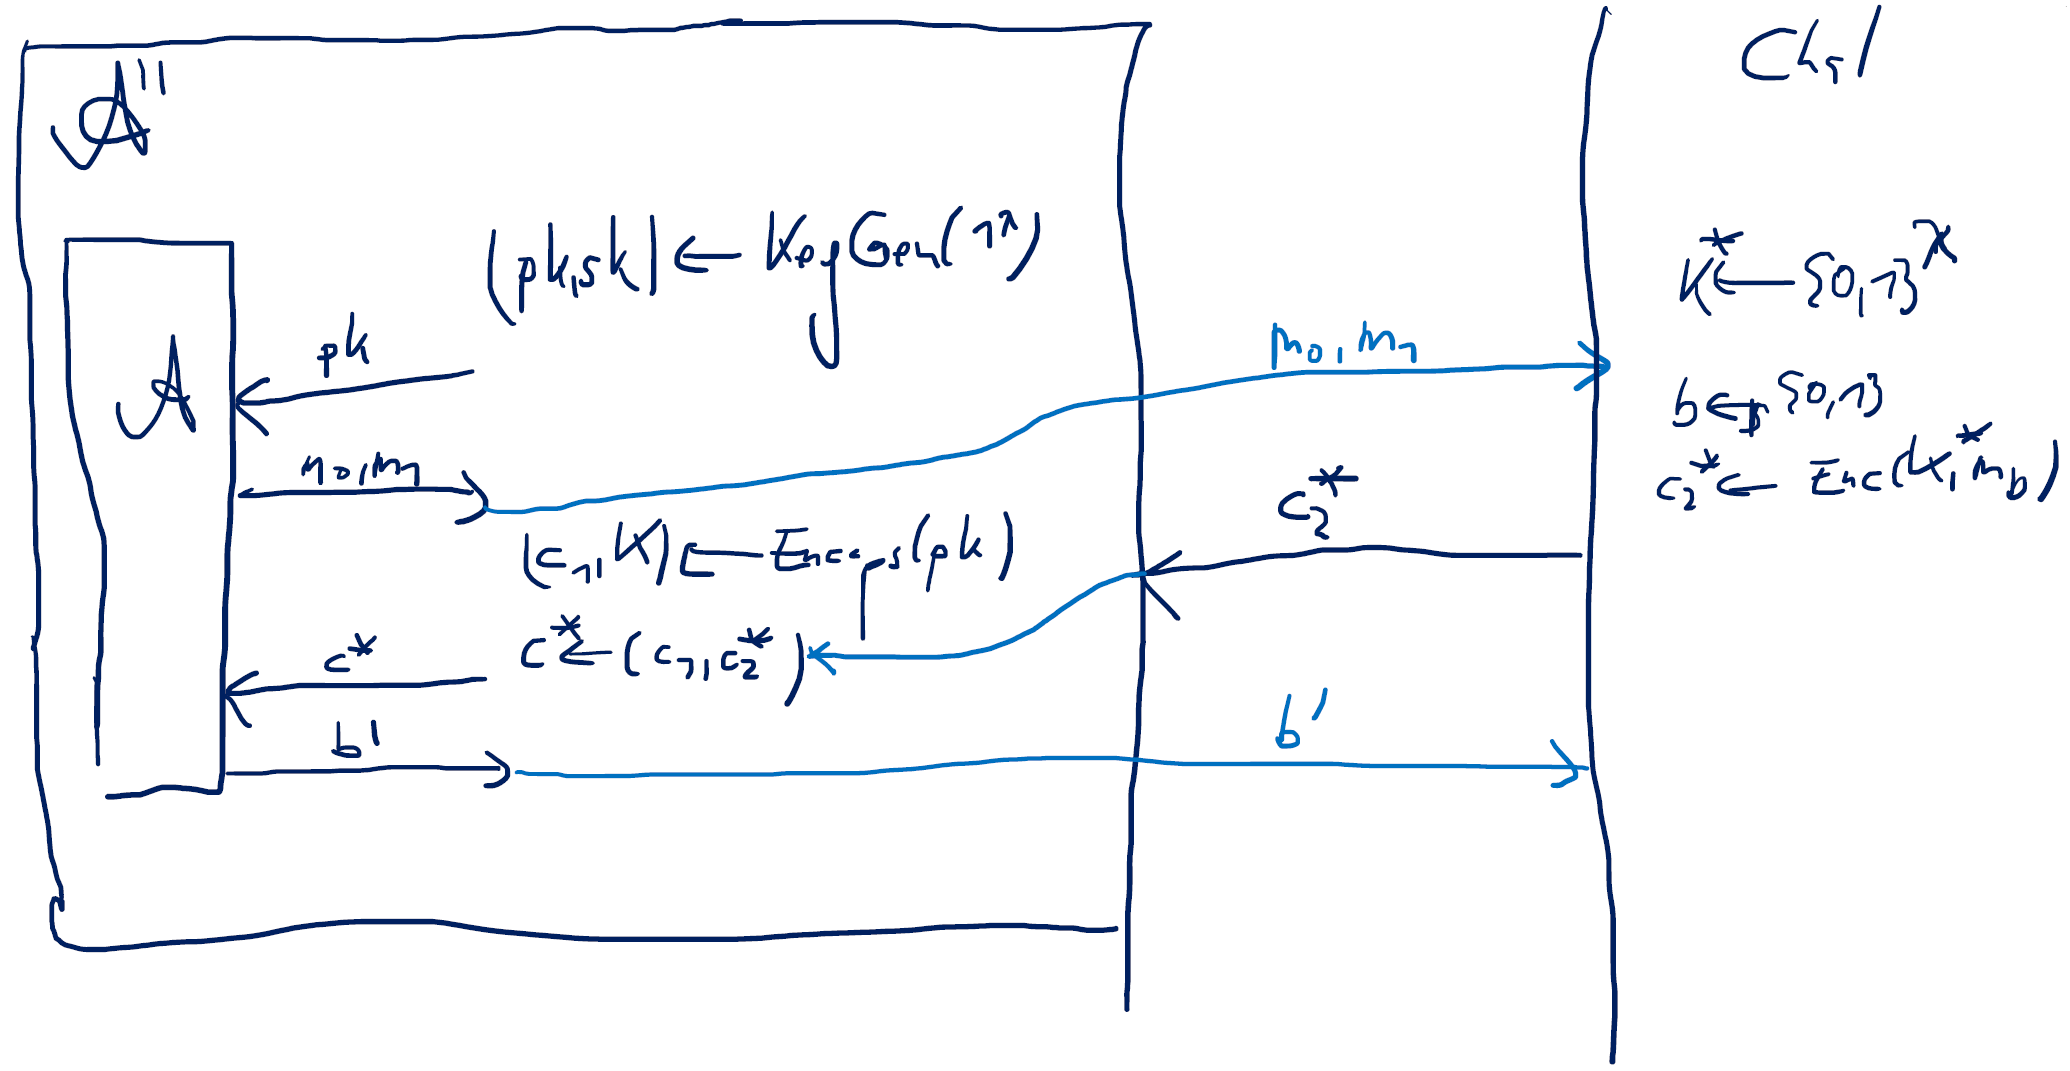
\includegraphics[width=160mm]{Graphics/Hybrid Encryption/he7.png}
    	\end{center}
    	From the view of $\mathcal{A}$, $\mathcal{A}''$ simulates $Exp'$ faithfully.
    	It follows that
    	    $$Pr[IND_{\mathcal{A}''}=1] = Pr[Exp'=1] \geq \frac{1}{2} + \epsilon''$$
        But this contradicts $IND$-security of $(Enc,Dec)$.
    \end{proof}

\section{Summary}
    \begin{itemize}
        \item Hybrid Encryption combines the advantages of public and private key encryption
        \item Public key part is only used to transport a key
        \item Payload message is encrypted under private key encryption scheme
        \item For long messages (e.g. movies), this is essentially as efficient as private key encryption
        \item Both in terms of ciphertext rate and encryption overhead
        \item Key encapsulation mechanisms (KEMs) provide an efficient way to encrypt a random key
    \end{itemize}




